\subsubsection{Quality-latency trade-Off}
\label{sec:streaming.results.quality}
In this section,
we present the translation quality and latency of the \seamlessstreaming Model.
Because \seamlessstreaming can process two modalities at the same time, we report results for both speech-to-text and speech-to-speech translations.
We only report the model trained with a set of loss weight hyperparameters.
The full results and metrics per evaluation direction can be found at \url{https://github.com/facebookresearch/seamless_communication}.


By default, we set decision threshold $t_{\emma}$ as 0.5 in \Cref{algo:streaming.inference},
which is also the default of EMMA model.
We then adjusted latency at a granular level by changing $t_{\emma}$.
We followed the post processing in \Cref{sec:offline:results} when computing BLEU scores on translation.
When evaluating the streaming models,
we removed the starting and ending silence in the source audio to follow real life setting.

We first present the speech-to-text results on \fleurs, shown in \Cref{tbl:streamin_s2t.latency-quality}.
We report averaged all the quality and latency under on $t_{\emma}$ setting.
To make latency comparable across different languages,
we evaluated average lagging (AL) and length-adaptive average lagging (LAAL) based on SentencePiece \citep{sentencepiece} tokens. %

\begin{table}[!tbh]
    \centering
    \small
    \begin{tabular}{@{}lccccccc@{}}
        \toprule
         \multirow{3}{*}{\bf Model}  
         &\multirow{3}{*}{\makecell[c]{{\bf Decision} \\\bf{Threshold}}}  
         & \multicolumn{3}{c}{\makecell[c]{\xeng \\{\it (n=101)}}} 
         & \multicolumn{3}{c}{\makecell[c]{\engx \\{\it (n=87)}}} \\
         \cmidrule(r){3-5}\cmidrule(l){6-8}
         & &  $\uparrow$BLEU & $\downarrow$AL & $\downarrow$LAAL & $\uparrow$BLEU & $\downarrow$AL & $\downarrow$LAAL\\
        \midrule
        \mfourttwo  &  & 23.7 & & & 22.2&  &  \\\midrule
        \multirow{4}{*}{\seamlessstreaming}  
 & 0.4 & 19.8 & 1.59 & 2.12 & 19.5 & 1.91 & 2.07 \\
 & 0.5 & 20.0 & 1.68 & 2.20 & 19.7 & 1.98 & 2.12 \\
 & 0.6 & 20.1 & 1.75 & 2.27 & 19.8 & 2.03 & 2.18 \\
 & 0.7 & 20.3 & 1.84 & 2.35 & 19.8 & 2.10 & 2.24 \\
        \bottomrule
    \end{tabular}
    \caption{Average translation quality and latency for the text output of \seamlessstreaming under different latency decision threshold $t_{\emma}$.}
    \label{tbl:streamin_s2t.latency-quality}
\end{table}

We also report the ASR performance of \seamlessstreaming in \Cref{tbl:streamin_asr.latency-quality}. 
Compared with S2TT task,
\seamlessstreaming can perform the ASR task with much lower latency, with less than 10 WER degradation from \mfourttwo. 
\begin{table}[!tbh]
    \centering
    \small
    \begin{tabular}{@{}lcccc@{}}
        \toprule
         \multirow{2}{*}{\bf Model}  &   \multirow{2}{*}{\makecell[c]{{\bf Decision} \\  \bf{Threshold}}}  & \multicolumn{3}{c}{\makecell[c]{\fleurs-90 \\ {\it (n=90)}}}  \\
         \cmidrule(r){3-5}
         & & $\downarrow$WER & $\downarrow$AL & $\downarrow$LAAL  \\
        \midrule
        \mfourttwo  &  & 23.8 &  & \\\midrule
        \multirow{4}{*}{\seamlessstreaming}  
 & 0.4 & 31.3 & 1.19 & 1.45 \\
 & 0.5 & 31.1 & 1.23 & 1.48 \\
 & 0.6 & 31.1 & 1.26 & 1.51 \\
 & 0.7 & 30.9 & 1.29 & 1.54 \\
        \bottomrule
    \end{tabular}
    \caption{Average translation quality and latency for the ASR output of \seamlessstreaming under different latency decision threshold $t_{\emma}$.} %
    \label{tbl:streamin_asr.latency-quality}
\end{table}


We then present the speech-to-speech results on \fleurs, shown in \Cref{tbl:streamin_s2s.latency-quality}.
The difference of the quality of speech output quality between \mfourttwo and \seamlessstreaming is bigger than text output in \Cref{tbl:streamin_s2t.latency-quality}. 
This part off the drop came from the discontinuity in the generated speech.
\begin{table}[!ht]
    \centering
    \small
    \begin{tabular}{@{}lccccc@{}}
        \toprule
         \multirow{3}{*}{\bf Model}  &   \multirow{3}{*}{\makecell[c]{{\bf  Decision} \\  \bf{Threshold}}}  & \multicolumn{2}{c}{\makecell[c]{\xeng \\{\it (n=101)}}} & \multicolumn{2}{c}{\makecell[c]{\engx\\{\it (n=35)}}} \\
         \cmidrule(r){3-4}\cmidrule(l){5-6}
         & & $\uparrow$ASR-BLEU & $\downarrow$\makecell[c]{Ending \\ Offset} & $\uparrow$ASR-BLEU & $\downarrow$\makecell[c]{Ending \\ Offset} \\
        \midrule
        \mfourttwo  &  & 29.7 &  & 26.1  \\\midrule
     \multirow{4}{*}{\seamlessstreaming}  
 & 0.4 & 21.8 & 2.66 & 20.8 & 4.59 \\
 & 0.5 & 22.1 & 2.79 & 21.4 & 4.64 \\
 & 0.6 & 22.0 & 2.82 & 21.5 & 4.69 \\
 & 0.7 & 22.1 & 2.90 & 21.6 & 4.73 \\
        \bottomrule
    \end{tabular}
    \caption{Average translation quality and latency for the speech output of \seamlessstreaming under different latency decision threshold $t_{\emma}$.}
    \label{tbl:streamin_s2s.latency-quality}
\end{table}

\subsubsection{Data resources}
Similar to most data-driven models,
the quality of the simultaneous policy and translation accuracy on certain language pair is related to the amount of the training data.
We show the percentage of BLEU score drop of the model from the offline \mfourttwo large and latency under different setting, in \Cref{tbl:streamin_s2t.resource} for text output and \Cref{tbl:streamin_s2s.resource} for speech output.

We observe that in both speech and text output,
high resource languages have smaller quality drop from offline \mfourttwo.
Furthermore, the latency on high resource languages are also smaller, especially under \xeng setting.

In zero-shot setting, we can see a significant drop in translation quality.
We can also see very small average lagging under the zero-shot setting.
A small average lagging and big quality drop indicate the model has over generation issue under such setting.

\begin{table}[!ht]
    \centering
    \small
    \begin{tabular}{@{}lcccccc@{}}
        \toprule
          \multirow{2}{*}{\makecell[c]{{\bf Resource Level}} } & \multicolumn{3}{c}{\makecell[c]{\xeng \\{\it (n=101)}}} & \multicolumn{3}{c}{\makecell[c]{\engx \\{\it (n=87)}}} \\
          \cmidrule(r){2-4}\cmidrule(l){5-7}
          & $\downarrow$ BLEU loss (\%)  &  $\downarrow$ AL &  $\downarrow$ LAAL &  $\downarrow$ BLEU loss (\%)   & AL &  $\downarrow$ LAAL \\
             \midrule
High & 10.1 & 1.75 & 2.08 & 10.5 & 1.94 & 2.06 \\
Medium & 14.8 & 2.09 & 2.40 & 13.1 & 1.97 & 2.11 \\
Low & 21.5 & 1.89 & 2.30 & 17.9 & 2.00 & 2.16 \\
Zero-Shot & 31.4 & 0.44 & 1.74 & 23.3 & 1.97 & 2.18 \\
        \bottomrule
    \end{tabular}
    \caption{Average translation drop from \mfourttwo large and latency for languages in different resource setting for speech-to-text task, $t_{\emma}=0.5$ }
    \label{tbl:streamin_s2t.resource}
\end{table}


\begin{table}[!tbh]
    \centering
    \small
    \begin{tabular}{@{}lcccc@{}}
        \toprule
          \multirow{3}{*}{\makecell[c]{{\bf Resource Level}} }  & \multicolumn{2}{c}{\makecell[c]{\xeng \\{\it (n=101)}}} & \multicolumn{2}{c}{\makecell[c]{\engx \\{\it (n=35)}}} \\
         \cmidrule(r){2-3}\cmidrule(l){4-5}
          & $\downarrow$ ASR BLEU loss (\%) & $\downarrow$ \makecell[c]{Ending \\ Offset} & $\downarrow$ ASR BLEU loss (\%)  & $\downarrow$ \makecell[c]{Ending \\ Offset} \\
       \midrule
High & 16.0 & 2.25 & 19.7 & 3.68 \\
Medium & 19.6 & 2.45 & 13.1 & 4.03 \\
Low & 20.7 & 2.61 & 26.7 & 4.15 \\
Zero-Shot & 20.2 & 2.20 & --- & --- \\
        \bottomrule
    \end{tabular}
    \caption{Average translation drop from \mfourttwo large and latency for languages in different resource setting for speech-to-speech task, $t_{\emma}=0.5$}
    \label{tbl:streamin_s2s.resource}
\end{table}



\paragraph{Language family.}
The quality of streaming translation varies with language pairs due to linguistic divergence, 
cultural disparities, and speech speed. Intuitively, close language relationships and shared cultural contexts ease streaming translation , while vast linguistic gaps, dissimilar syntax, and unfamiliar cultural nuances pose challenges.

Because \seamlessstreaming is trained on English centered data,
we also investigate the its performance when translate from or into different language families.
We show the average quality and average lagging under different language subgroups then translated from or input English, in \Cref{fig:streaming_s2t.language_family} for text output and \Cref{fig:streaming_s2t.language_family} for speech output.
We only show the results on high resource languages in the figure to avoid the sub-optimized simultaneous policy due to the lack of data.

In both text and speech output,
into and from English directions,
the model has better translation quality and lower average lagging in ``Italic'' (e.g. Spanish, French, Portuguese, Italian, and Romanian) and ``Germanic'' (e.g. German, Dutch) languages,
which considers to be close to English.
On the contrary,
in distant language subgroups compared with English,
such as ``Sinitic'' (e.g. Chinese Mandarin, Chinese Yue), ``Japanesic'' (e.g. Japanese) and ``Indo-Aryan'' (e.g  Hindi, Urdu, Bengali),
are observed bigger drop of translation quality and increased average lagging.



\begin{figure}[!th]
    \centering
    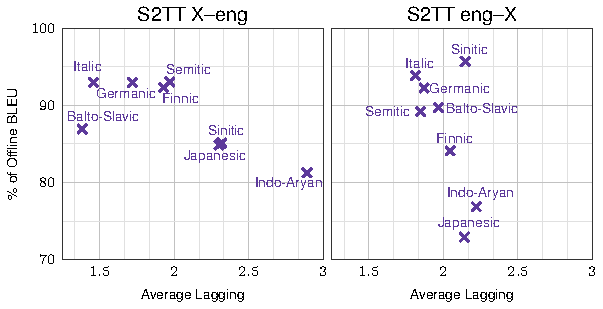
\includegraphics[width=.7\linewidth]{figures/streaming/s2t_quality_lagging_treadeoff.pdf}
    \caption{Average quality and average lagging of text output (\st) over different language subgroups, translated from and into English; $t_{\emma}=0.5$}
    \label{fig:streaming_s2t.language_family}
\end{figure}
\begin{figure}[!ht]
    \centering
    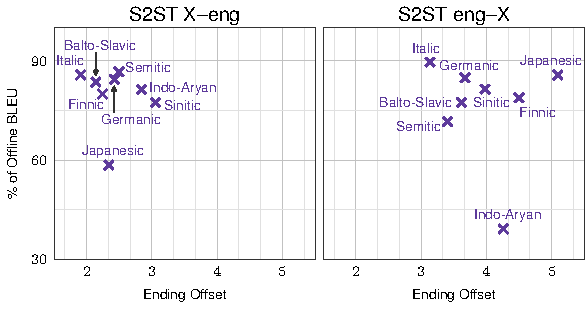
\includegraphics[width=0.7\linewidth]{figures/streaming/s2s_quality_offset_treadeoff.pdf}
    \caption{Average quality and average lagging of speech output (\sst) over different language subgroups, translated from and into English; $t_{\emma}=0.5$}
    \label{fig:streaming_s2s.language_family}
\end{figure}